% Generated by tools/pipeline/figures.py from a1_dryrun_20260905b/metrics.json. Do not edit by hand.
\begin{figure}[htbp]
\centering
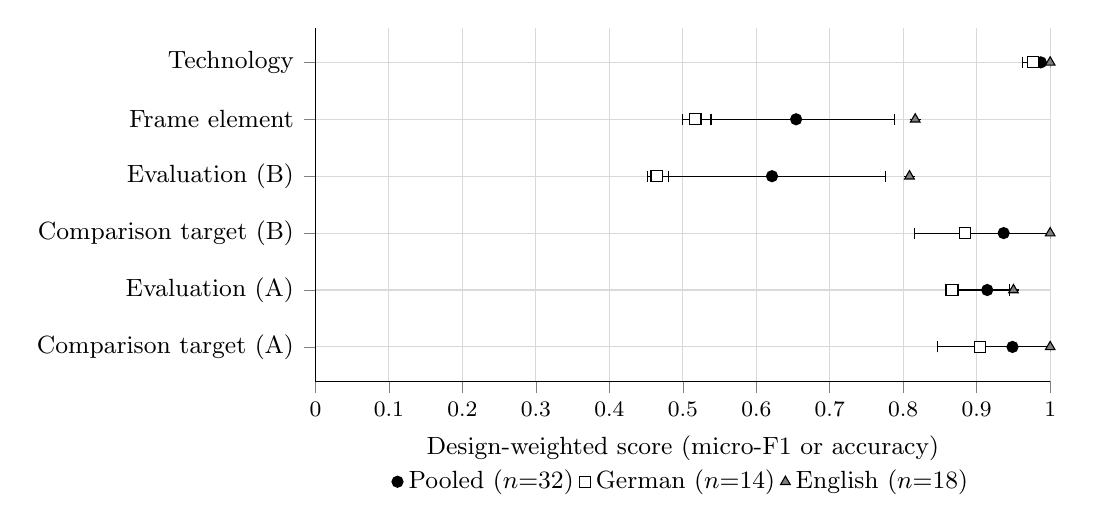
\begin{tikzpicture}
\begin{axis}[
  width=0.9\textwidth, height=0.5\textwidth,
  xmin=0, xmax=1, xlabel={Design-weighted score (micro-F1 or accuracy)}, xlabel style={font=\small},
  symbolic y coords={{Technology},{Frame element},{Evaluation (B)},{Comparison target (B)},{Evaluation (A)},{Comparison target (A)}}, ytick=data, y dir=reverse,
  yticklabel style={font=\small}, xticklabel style={font=\footnotesize},
  legend style={at={(0.5,-0.22)}, anchor=north, legend columns=3, font=\small, draw=none, fill=none},
  legend cell align=left, axis lines*=left, tick align=outside,
  enlarge y limits=0.12, grid=major, grid style={black!15},
]
\addplot[only marks, mark=*, mark options={fill=black, draw=black}, error bars/.cd, x dir=both, x explicit] coordinates {(0.9873,{Technology}) -= (0.0244,0) += (0.0127,0) (0.6542,{Frame element}) -= (0.1542,0) += (0.1344,0) (0.6214,{Evaluation (B)}) -= (0.1697,0) += (0.1544,0) (0.9367,{Comparison target (B)}) -= (0.1219,0) += (0.0633,0) (0.9143,{Evaluation (A)}) -= (0.0571,0) += (0.0298,0) (0.9487,{Comparison target (A)}) -= (0.1026,0) += (0.0513,0)};
\addplot[only marks, mark=square*, mark options={fill=white, draw=black}, error bars/.cd, x dir=both, x explicit] coordinates {(0.9767,{Technology}) -= (0.0138,0) += (0.0233,0) (0.5172,{Frame element}) -= (0.0172,0) += (0.0212,0) (0.4643,{Evaluation (B)}) -= (0.0127,0) += (0.0157,0) (0.8837,{Comparison target (B)}) -= (0.0689,0) += (0.1163,0) (0.8667,{Evaluation (A)}) -= (0.0095,0) += (0.0083,0) (0.9048,{Comparison target (A)}) -= (0.0586,0) += (0.0952,0)};
\addplot[only marks, mark=triangle*, mark options={fill=black!50, draw=black}, error bars/.cd, x dir=both, x explicit] coordinates {(1.0000,{Technology}) -= (0.0000,0) += (0.0000,0) (0.8163,{Frame element}) -= (0.0000,0) += (0.0000,0) (0.8085,{Evaluation (B)}) -= (0.0000,0) += (0.0000,0) (1.0000,{Comparison target (B)}) -= (0.0000,0) += (0.0000,0) (0.9500,{Evaluation (A)}) -= (0.0000,0) += (0.0000,0) (1.0000,{Comparison target (A)}) -= (0.0000,0) += (0.0000,0)};
\legend{{Pooled ($n$=32)},{German ($n$=14)},{English ($n$=18)}}
\end{axis}
\end{tikzpicture}
\caption{Headline agreement between the model's first execution and the human reference, by scoring dimension and population. Marks are design-weighted point estimates; bars are the 2.5--97.5 percentile interval over 500 article resamples. Run \texttt{a1\_dryrun\_20260905b}.}
\label{fig:primary}
\end{figure}
